
\documentclass[10pt, a4paper, twoside]{article}
\usepackage[utf8]{inputenc}
\usepackage{newtxtext,newtxmath} % Times New Roman font
\usepackage[left=2.54cm, right=2.54cm, top=2.54cm, bottom=2.54cm, headheight=15pt]{geometry}
\usepackage{titlesec} % For customizing section titles
\usepackage{enumitem} % Enables bullet points
\usepackage{lipsum} % Add dummy text
\usepackage{hyperref} % Links for references
\usepackage{parskip} % Set spacing between paragraphs
\usepackage{fancyhdr} % Format headers
\usepackage{etoolbox} % Format bibliography header
\usepackage{siunitx} % Used to write SI base units
\usepackage{physics} % Used to write differential equations more easily
\usepackage{graphicx} % Used for figures
\usepackage{caption} % Used to edit the figure captions

% This code is used to supress \qty warning conflict between siunitx and physics packages
\ExplSyntaxOn
\msg_redirect_name:nnn { siunitx } { physics-pkg } { none }
\ExplSyntaxOff

\setlength{\parskip}{10pt}

\titleformat{\section}{\normalfont\fontsize{10}{13}\uppercase}{\thesection.}{1em}{}
\titleformat{\subsection}{\normalfont\fontsize{10}{13}\bfseries}{\thesubsection.}{1em}{}
\titleformat{\subsubsection}{\normalfont\fontsize{10}{13}\itshape}{\thesubsubsection.}{1em}{}

% Redefining \section* command for centered section title
\titleformat{name=\section,numberless}{\normalfont\fontsize{10}{13}\bfseries\centering\uppercase}{}{0pt}{}

% Ensure references title has the same format as \section*
\patchcmd{\thebibliography}{\section*{\refname}}{\section*{REFERENCES}}{}{}

%  Create headers and footers
\fancyhf{} % clear all header and footer fields
\renewcommand{\headrulewidth}{0pt}
\fancyhead[CE]{\fontsize{8}{10}\selectfont \textbf{IAEA-CN-316/2143}}
\fancyhead[CO]{\fontsize{8}{10}\selectfont \textbf{PROKOPYSZYN et al.}}
\fancyfoot[RO]{\fontsize{10}{13}\selectfont \thepage}
\pagestyle{fancy}
% \pagestyle{plain}

% Set the caption font size to 9pt
\DeclareCaptionFont{ninept}{\fontsize{9pt}{12pt}\selectfont}
\renewcommand{\figurename}{\textit{FIG.}}
\captionsetup{
    justification=raggedright,
    singlelinecheck=true,
    font=ninept,
    textfont=it,
    labelfont=it,
    labelsep=period,
    labelformat=simple,
    format=hang
}

\begin{document}
\begin{flushleft}
\fontsize{12}{14}\selectfont \textbf{CONFINEMENT OF FUSION ALPHA-PARTICLES AND ALFV\'EN EIGENMODE STABILITY IN STEP}
% \fontsize{12}{14}\selectfont \textbf{\textit{Subtitle if needed in Times New Roman 12 point bold italic, sentence case}}

\fontsize{10}{13}\selectfont
A.P.K. PROKOPYSZYN, K.G. MCCLEMENTS, H.J.C. OLIVER, M. FITZGERALD, D.A. RYAN, G. XIA \\
United Kingdom Atomic Energy Authority \\
Culham Centre for Fusion Energy, Culham Science Centre, Abingdon, Oxfordshire OX14 3DB, United Kingdom \\
Email: alex.prokopysyzn@ukaea.uk

\end{flushleft}

% Abstract section
\begin{flushleft}
\textbf{Abstract}
\end{flushleft}

\setlength{\parindent}{1cm}
\fontsize{9}{12pt}\selectfont

The Spherical Tokamak for Energy Production (STEP) programme is focused on constructing a fusion power plant prototype that will generate approximately 1.5-1.7 GW of deuterium-tritium fusion energy. To achieve this, the $\alpha$-particles generated through fusion must be adequately confined to maintain the necessary high temperature in the core of the plasma and to protect the wall from too much damage. Microwaves will be used for both external heating and current drive, making $\alpha$-particles the only significant fast-ion species. The purpose of this work is to model the confinement of $\alpha$-particles and the toroidal Alfvén eigenmodes (TAEs) driven by these particles in a variety of scenarios to help determine the best configuration. The scenarios examined here have been identified by the STEP team as potential flat-top operating configurations. We use LOCUST (Lorentz Orbit Code for Use in Stellerators and Tokamaks) to model the $\alpha$-particle confinement and heat-load distribution on the wall, and HALO (HAgis LOcust) to model the TAEs. The results indicate that adequate confinement can be achieved in candidate flat-top operating points, but the results are sensitive to some of the system parameters. For instance, a change in the phase difference between upper and lower edge localised mode (ELM) suppression coils can increase the peak first wall power loading due to $\alpha$-particle losses by a factor of ten.

% Abstract and title over, format text for the main body
\setlength{\parindent}{0pt}
\fontsize{10}{13}\selectfont

\section{Introduction}
\label{sec:introduction}

UKAEA is pioneering efforts to develop a compact prototype of a fusion energy power plant and establish a commercial pathway for fusion energy \cite{nuttall2020, meyer2023, mitchell2023}. A crucial factor in the viability of a deuterium-tritium (D-T) burning fusion reactor is the confinement of fusion-born $\alpha$-particles since, in addition to providing most of the plasma heating, these particles have the potential to damage the reactor walls when unconfined. Ideally, $\alpha$-particles should slow down through Coulomb collisions with thermal electrons and ions while undergoing a modest level of (purely collisional) transport. However, they can drive high-frequency instabilities that may in turn transport them at rates that are well above collisional levels \cite{garcia-munoz2011}. Toroidal Alfv\'en eigenmodes (TAEs) exemplify the type of fast particle-driven instability that can significantly disrupt plasma confinement. In the present work we model $\alpha$-particle losses in the presence of static magnetic fields and determine the stability of TAEs in candidate STEP plasmas with the objective of informing the design process for this device.

For safety and economic reasons, the plasma-facing components (PFCs) must contain the plasma and be highly durable to prevent frequent damage. During operation, the PFCs will be exposed to heat from various sources, even if disruptions are successfully avoided. The wall will be exposed to electromagnetic radiation from the plasma, neutrons, thermal charged particles, runaway electrons, erosion due to sputtering, and $\alpha$-particles. Here, we consider the contribution of $\alpha$-particles. See, for example, \cite{bachmann2018} for a discussion {\it inter alia} of the heat loads on PFCs in a conventional tokamak reactor and \cite{fil2023} for an overview of the modeling of runaway electrons for STEP. Our objective is to maintain the heat load on the wall at a level less than approximately $1\, \text{MWm}^{-2}$ on the first wall of the main chamber, about $5\, \text{MWm}^{-2}$ on dome structures in the divertor regions, and $10\, \text{MWm}^{-2}$ on the divertors themselves. It is important to note that our wall, while incorporating limiters, remains smooth and axisymmetric, although the final design will be comparatively less smooth. Consequently, we must achieve lower heat loads to compensate for shadowing, which can increase the peak heat load.

Because of their large Larmor radii, the confinement of $\alpha$-particles can easily be compromised due to deviations in the background magnetic field from axisymmetry.  In this study, we model $\alpha$-particles in fields that are axisymmetric except for two types of three-dimensional perturbation. The first of these stems from the ripple introduced by the use of a finite number of toroidal field (TF) coils. The second arises from coils that generate resonant magnetic perturbations (RMPs) aimed at suppressing edge-localized modes (ELMs) \cite{zohm1996}.

STEP will need to operate in high-confinement mode (H-mode), and therefore type-I ELMs may pose a significant problem. ELM suppression using RMP coils has been successfully experimentally demonstrated in medium-sized conventional tokamaks such as ASDEX Upgrade \cite{suttrop2018}. However, the nonaxisymmetric RMP fields violate conservation of fast-ion toroidal canonical momentum, and can thus deconfine these ions. The effects of RMPs on fast ions have been studied in DIII-D, ASDEX Upgrade, and ITER \cite{van2015,sanchis2018,ward2022}. Currently, there is no definitive set of criteria for ELM suppression. Therefore, the ELM suppression coils for STEP should be flexible enough to experimentally determine an optimal configuration, and it is necessary to model $\alpha$-particle losses for a range of RMP scenarios.
We only consider the plasma during the flat-top phase as $\alpha$-particle production will be negligible for the greater part of the ramp-up and ramp-down phases. In order to accurately model the $\alpha$-particles we require profiles of temperature and density as well as the magnetic field. These profiles have been determined using the integrated modelling suite JINTRAC \cite{meyer2023, mitchell2023}. This sophisticated tool incorporates a wide range of physics processes, including simplified fast-ion models, providing a comprehensive basis for our analysis.

The structure of this paper is as follows. Section\ref{sec:locust_work} details our efforts using the LOCUST code to model $\alpha$-particle in the flat-top and compute the associated heat load on the wall. In this section, background quantities, such as the magnetic field, are held constant. In Section \ref{sec:halo_work} we consider the magnetic field's response to the presence of $\alpha$-particles and assess TAE stability using the HALO code. In Section \ref{sec:discussion_and_conclusions}, we summarise our findings and discuss their implications.

\section{Alpha particle confinement}
\label{sec:locust_work}

Our purpose in this section is to calculate the $\alpha$-particle flux that strikes the walls of STEP and to determine the location and magnitude of the peak flux. To gain a better understanding of how our results are affected by different design choices and parameters, we have run simulations with varying parameters and analysed the particle losses. This analysis is beneficial in the design process, allowing us to identify scenarios that minimise the heat load on the reactor walls.

\subsection{Model}

We calculate the $\alpha$-particle energy flux on the walls of STEP using the LOCUST code (see \cite{akers2018, ward2021} for a more comprehensive explanation of how it works). This tracks particles, represented by markers, which represent samples of the $\alpha$-particle distribution. These markers are traced from birth until they escape and collide with PFCs, or their energy drops below a threshold equal to 1.5 times the bulk ion temperature, at which point they are considered to have thermalised.

We represent the position of the $j^{\text{th}}$ marker at time $t$ by $\mathbf{x}_j(t)$, and denote
the background magnetic field at the position of the marker by $\textbf{B}(\mathbf{x}_j)$.
The forces on the marker due to collisions with the background ions and electrons are $\textbf{F}_{\alpha,i}(\mathbf{x}_j)$ and $\textbf{F}_{\alpha,e}(\mathbf{x}_j)$ respectively, while the mass and charge of the $\alpha$-particles are $m_\alpha$ and $q_\alpha$ respectively. The equation of motion for the $j^{\text{th}}$ marker is
\begin{equation}
m_\alpha\dv[2]{\mathbf{x}_j}{t} = q_\alpha\dv{\mathbf{x}_j}{t}\cross\textbf{B}(\mathbf{x}_j) + \textbf{F}_{\alpha,i}(\mathbf{x}_j) + \textbf{F}_{\alpha,e}(\mathbf{x}_j).
\end{equation}

We do not consider collisions between fast $\alpha$-particles, an omission that is justified by the low concentration of this species, and consequently each $\alpha$-particle is modelled independently. This approach presents substantial computational advantages as it allows for parallel processing. To capitalise on this, LOCUST utilises GPU architecture, enabling the simultaneous modelling of very large numbers of particles. This approach is computationally more efficient and cost-effective than CPU-based modelling. We randomly select the initial positions and velocities. The positions are determined by a probability distribution shaped by the Bosch-Hale D-T reaction rate \cite{bosch1992}. We model the birth velocity distribution as isotropic, setting the mean kinetic energy at 3.5 MeV with a spread of about 6\% \cite{brysk1973}. We use the most recent design of the first wall for this investigation. The design of the wall, particularly the divertor region, is still being developed, with further iterations expected. The current model does not include details of the eventual design, such as boundaries between the tiles covering the final wall. Our model features a smooth surface, which means that the shadowing effects of the tiles are neglected. The model wall is mainly axisymmetric, but three rows of limiters have been added, eight on the top and bottom rows, and four in the midplane. The axisymmetric component of the magnetic field was calculated using the free boundary FIESTA code. 

At the end of a LOCUST simulation we calculate the power lost to the first wall using the expression 
\begin{equation} 
P_{lost} = P_\alpha \frac{\sum_{j\in \text{\{set of markers that hit the wall\}}}\abs{\textbf{v}_{\text{final}, j}^2}}{\sum_{j \in \{\text{set of all markers}\}} \abs{\mathbf{v}_{\text{initial}, j}^2 }}, 
\end{equation}
where $P_\alpha$ is the thermonuclear $\alpha$-particle power, equal to $\si{304.MW}$ in the present case. Additionally, $\mathbf{v}_{\text{final}, j}$ is the final velocity of the j\textsuperscript{th} marker upon hitting the wall, and $\mathbf{v}_{\text{initial}, j}$ is the birth velocity of the j\textsuperscript{th} marker.

To determine whether PFCs can withstand the impacts of the thermonuclear $\alpha$-particles, we need to know the energy flux of the $\alpha$-particles on the wall: this is not evenly distributed. We calculate the energy flux using kernel density estimation \cite{chen2017} and leave-one-out cross-validation \cite{chen2017} to determine the bandwidth. We also use bootstrap resampling to calculate 95\% confidence intervals for the maximum flux \cite{chen2017}.

\subsection{Results}

\subsubsection{TF ripple field}
\label{sec:tf_ripple_field}

It is expected that STEP plasmas will be highly elongated. The toroidal field (TF) coils of the current design are projected to be around $\si{22.m}$ tall and have a rectangular shape (see Fig. \ref{fig:coil_plot_3d}), although this may be altered in the future. Due to the coil geometry, the ripple field in the plasma, can be well-approximated by
% \begin{equation}
%     \label{eq:ripple_field}
%     \begin{aligned}
%         \delta B_R^{\text{ripple}}(R, \phi, z) &= \frac{B_0 R_0}{R} \qty(\frac{R}{R_{\text{coil}}})^{N_{coil}}\sin(N_{\text{coil}}\phi) +  O\qty[\frac{B_0 R_0}{R}\qty(\frac{R}{R_\text{coil}})^{2N_{\text{coil}}}], \\
%         \delta B_\phi^{\text{ripple}}(R, \phi, z) &= \frac{B_0 R_0}{R} \qty(\frac{R}{R_{\text{coil}}})^{N_{coil}}\cos(N_{\text{coil}}\phi)  +  O\qty[\frac{B_0 R_0}{R}\qty(\frac{R}{R_\text{coil}})^{2N_{\text{coil}}}]\\
%         \delta B_z^{\text{ripple}}(R, \phi, z) &= O\qty[\frac{B_0 R_0}{R}\qty(\frac{R}{R_\text{coil}})^{2N_{\text{coil}}}],
%     \end{aligned}
% \end{equation}
\begin{equation}
    \label{eq:ripple_field}
    \begin{aligned}
        \delta B_R^{\text{ripple}}(R, \phi, z) &\approx \frac{B_0 R_0}{R} \qty(\frac{R}{R_{\text{coil}}})^{N_{coil}}\sin(N_{\text{coil}}\phi), \\
        \delta B_\phi^{\text{ripple}}(R, \phi, z) &\approx \frac{B_0 R_0}{R} \qty(\frac{R}{R_{\text{coil}}})^{N_{coil}}\cos(N_{\text{coil}}\phi),\\
        \delta B_z^{\text{ripple}}(R, \phi, z) &\approx 0.
    \end{aligned}
\end{equation}
Here, $R$ denotes the major radius, $R_0$ is the major radius of the plasma's geometric center, $B_0$ represents the toroidal magnetic field when $R=R_0$, $N_{\text{coil}}$ is the count of TF coils, and $\phi$ gives the toroidal angle, expressed in radians. A derivation of Equation \eqref{eq:ripple_field} can be found in, for example, \cite{mcclements2005}.  When we compared Equation \eqref{eq:ripple_field} with the numerical predictions of the ripple field, the discrepancy was below 1\% on the outer side of the plasma. Furthermore, our simulations, using both methodologies, confirmed concordant results within the statistical error margins arising from the use of a finite number of markers.

\begin{figure}[!htb]
    \centering
    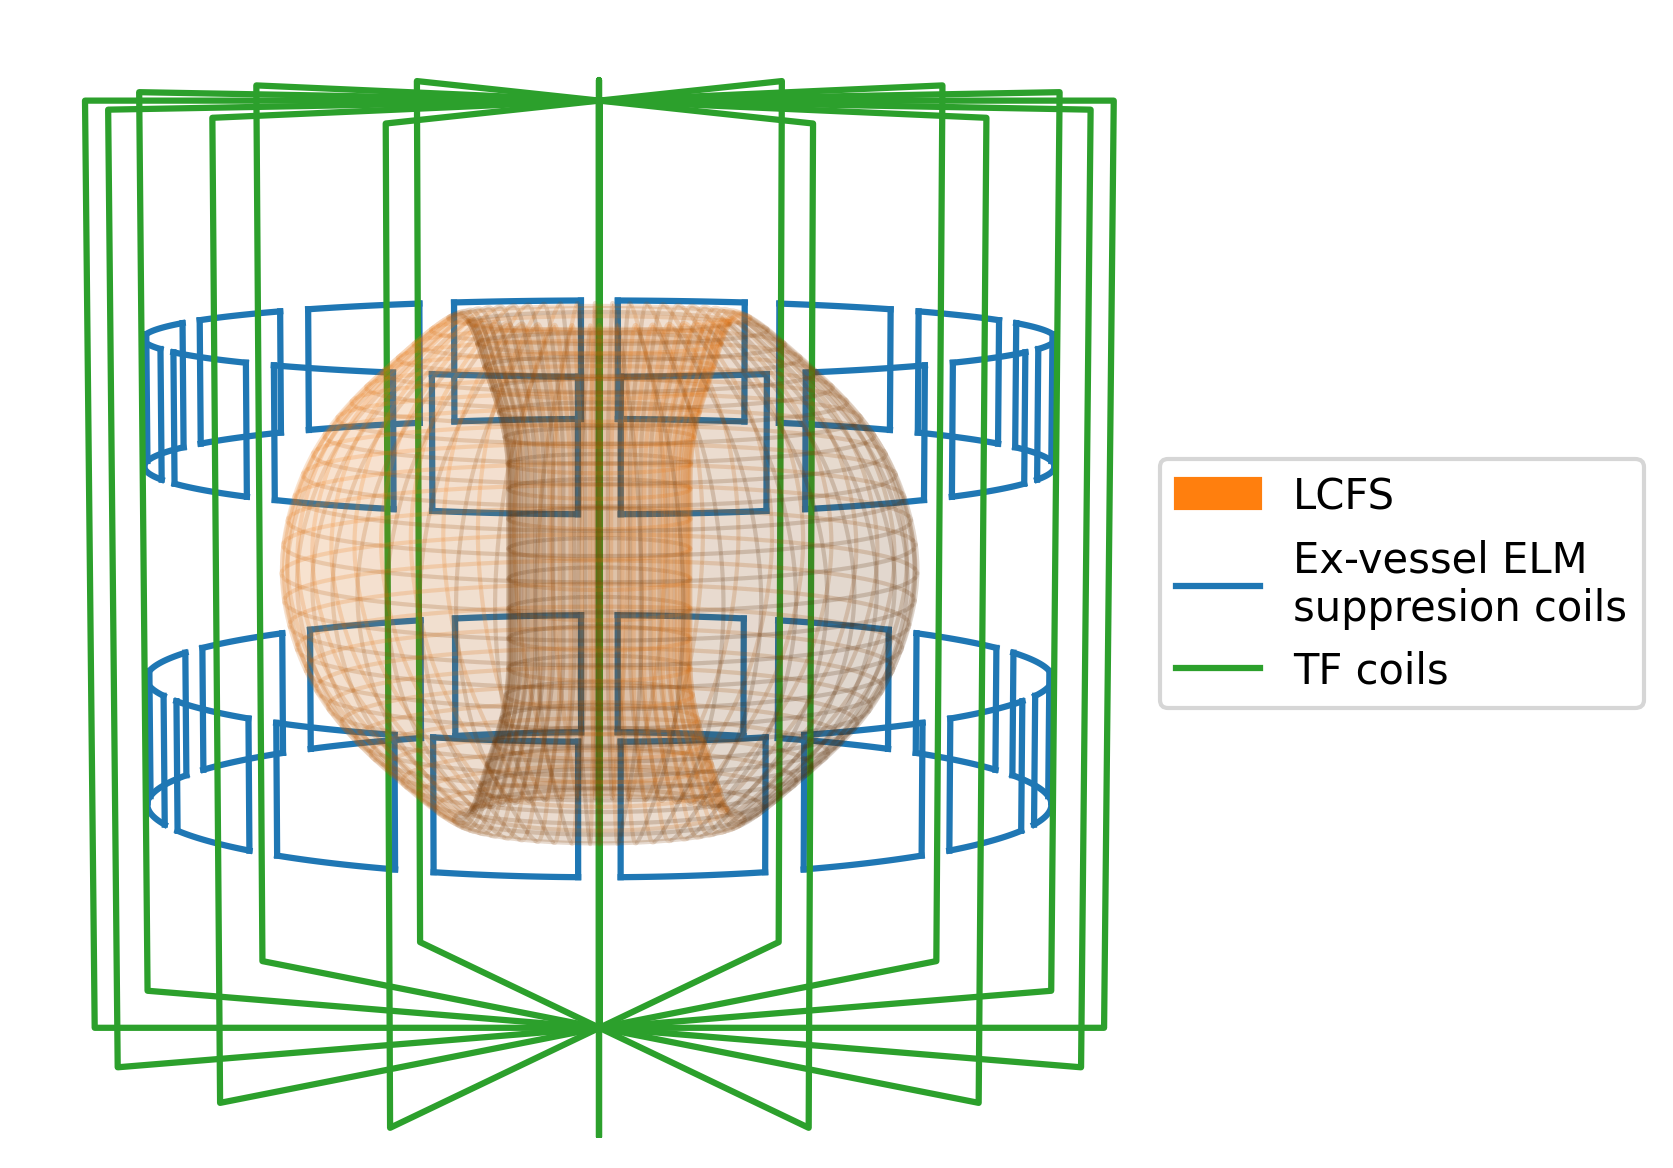
\includegraphics[width=0.6\linewidth]{Figures/coil_plot_3d.png}
    \caption{Schematic representation of STEP’s last closed flux surface (LCFS), ELM suppression coils (which are exterior to the vacuum vessel), and TF coils. These designs may change in the future. 
}
    \label{fig:coil_plot_3d}
\end{figure}

Fig. \ref{fig:max_and_total_flux_vs_rcoil_and_ncoil} shows the maximum energy flux on the walls and the total flux for different radii of the TF coils and the number of TF coils. The current design, with a major radius of approximately $\si{9.m}$ and 16 TF coils, has power losses that remain within acceptable limits. Increasing the radius of the coil or the number beyond these values will have a minimal effect on improving the confinement of the $\alpha$ particles. 
% Unfortunately, due to the need to fit other instruments such as the vacuum vessel, it is difficult to reduce the outer radius of the TF coil. The results also show that we can reduce the number of TF coils from 16 to 12 without affecting the confinment (assuming a radius of $9\si{.m}$ is maintained).
Unfortunately, it is difficult to reduce the outer radius of the TF coils due to the need to accommodate other essential elements such as the vacuum vessel, blanket, and PF (polodial field) coils. However, the results indicate that the number of TF coils could be reduced from 16 to 12 without compromising the confinement if a coil radius of $9\si{.m}$ were adopted.

\begin{figure}[!htb]
    \centering
    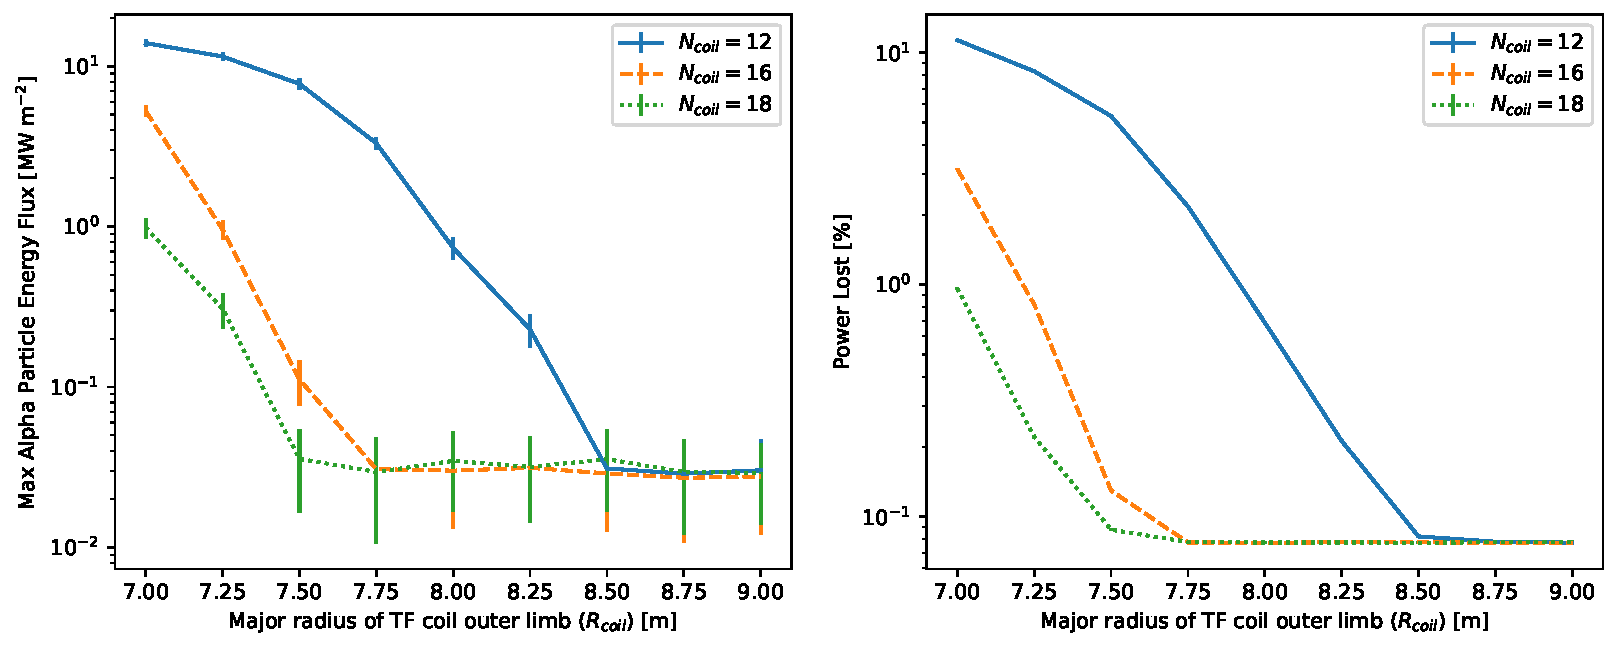
\includegraphics[width=0.99\linewidth]{Figures/max_and_total_flux_vs_rcoil_and_ncoil.pdf}
    \caption{TF ripple-induced losses for three values of $N_{\rm coil}=$, the number of TF coils. The left plot shows the maximum energy flux on the reactor wall in $\si{MW.m^{-2}}$ and the right plot indicates the percentage of $\alpha$-particle power escaping and impacting the PFCs. Error bars represent 95\% confidence intervals, reflecting the statistical uncertainty inherent in the Monte Carlo methodology of the simulation.}
    \label{fig:max_and_total_flux_vs_rcoil_and_ncoil}
\end{figure}

\subsubsection{ELM suppression field}
\label{sec:elm_suppression_field}

In this section, we model the confinement of $\alpha$-particles in the presence of the ELM suppression field, excluding the TF ripple component (the latter has a minimal effect on the confinement in the most recent TF coil design). The ELM suppression field we model is created by coils that are located outside the vacuum vessel (see Fig. \ref{fig:coil_plot_3d}) and are used to generate both the error field correction (EFC) field and the ELM suppression field. Although it is possible that resistive wall mode suppression coils located inside the vacuum vessel in the future may be used to generate the ELM suppression field, EFC coils are preferred in the current design. In the present design there are 16 such coils, but this could be reduced to 8.

The current in the $k^\text{th}$ coil, $I_k$, is given by
\begin{equation}
    \label{eq:ELM_coilcurrent_profile}
    I_k = I_0 \cos(n \phi_k + \Delta \phi),
\end{equation}
where $k$ ranges from 1 to 16, $I_0$ is the maximum current value, $\phi_k$ is the toroidal angle of the centre of the $k^\text{th}$ coil, $n$ is the toroidal mode number chosen to be excited, and $\Delta \phi$ is a free parameter that provides a phase shift. This produces a magnetic field that can be expressed as
\begin{equation}
    \delta\textbf{B}^\text{ELM}(R, \phi, z)=\Re\qty[\qty(\delta\textbf{B}^\text{ELM}_\text{real}(R,z) + i\delta\textbf{B}^\text{ELM}_\text{imag}(R,z))\exp[i(n\phi + \Delta \phi)]].
\end{equation}
Other toroidal harmonics (sidebands) are present, but they have a small enough amplitude that their effect on $\alpha$-particle confinement can be disregarded when 16 ELM suppression coils are used. However, if only 8 coils are employed, the sidebands cannot be ignored. The magnetic fields arising from these currents are in general modified as a result of their interaction with the plasma. The plasma's reaction is more prominent for lower toroidal mode numbers ($n$) \cite{mcclements2005}. For the ripple field, the plasma's response can be disregarded. For ELM suppression, we plan to set $n=3$. Greater values of $n$ decay more quickly with distance from the coils, decreasing their efficacy, while smaller values of $n$ may activate locked modes. See Equation \eqref{eq:ELM_coilcurrent_profile} Nevertheless, the choice of $n$ may change, and so we also model the cases with $n=2$ and $n=4$. To model the plasma response, we used the MARS-F code \cite{liu2015}. It is hard to confirm the accuracy of our plasma response calculations and so we will also analyse the results for the case where the vacuum ELM suppression field is used.

Equation \ref{eq:ELM_coilcurrent_profile} has three adjustable parameters: the toroidal mode number ($n$), the amplitude ($I_0$), and the phase shift $\Delta \phi$. We will consider the cases where $n$ is equal to 2, 3, and 4. To suppress ELMs, $I_0$ must be large enough, but not so large that it reduces $\alpha$-particle confinement to an unacceptable extent. Experiments on ASDEX Upgrade, when extrapolated to STEP, suggest that for $n=2$, a current of 50 kAt would be necessary, for $n=3$ a current of 90 kAt would be required, and for $n=4$ a current of 150 kAt would be needed. However, there is a high degree of uncertainty over the current needed, so we also model coil currents with twice these values. Additionally, we investigate the effect of varying the phase shift $\Delta\phi$ of the current profile of the lower coil set relative to the upper set on fast particle confinement. We consider $\Delta\phi =$ $0^\circ$, $45^\circ$, $90^\circ$, $135^\circ$, $180^\circ$, $225^\circ$, $270^\circ$, and $315^\circ$.

Fig. \ref{fig:max_and_total_flux_vs_phase} shows the predicted maximum flux of $\alpha$-particle energy on the wall of STEP and the percentage of $\alpha$-power lost, assuming 1.7 GW of fusion power (hence $\sim 338\,$MW of $\alpha$-particle power). The results are highly sensitive to the phase shift, as observed experimentally in ASDEX Upgrade \cite{sanchis2018}. Fig. \ref{fig:max_and_total_flux_vs_phase} also shows that the losses are greater when the plasma response to the ELM suppression field is taken into account. However even when larger coil currents are used and the plasma response is included, acceptable confinement can be achieved ($<1\si{.MW.m^{-2}}$) for suitably-chosen values of the phase shift. The findings suggest that better confinement can be achieved for $n=3$ and $n=4$ than for $n=2$. This could be due to the fact that higher toroidal modes decay more rapidly with distance from the coils, thus reducing the field perturbations in the plasma core where the great majority of high energy $\alpha$-particles are located.

\begin{figure}[!htb]
    \centering
    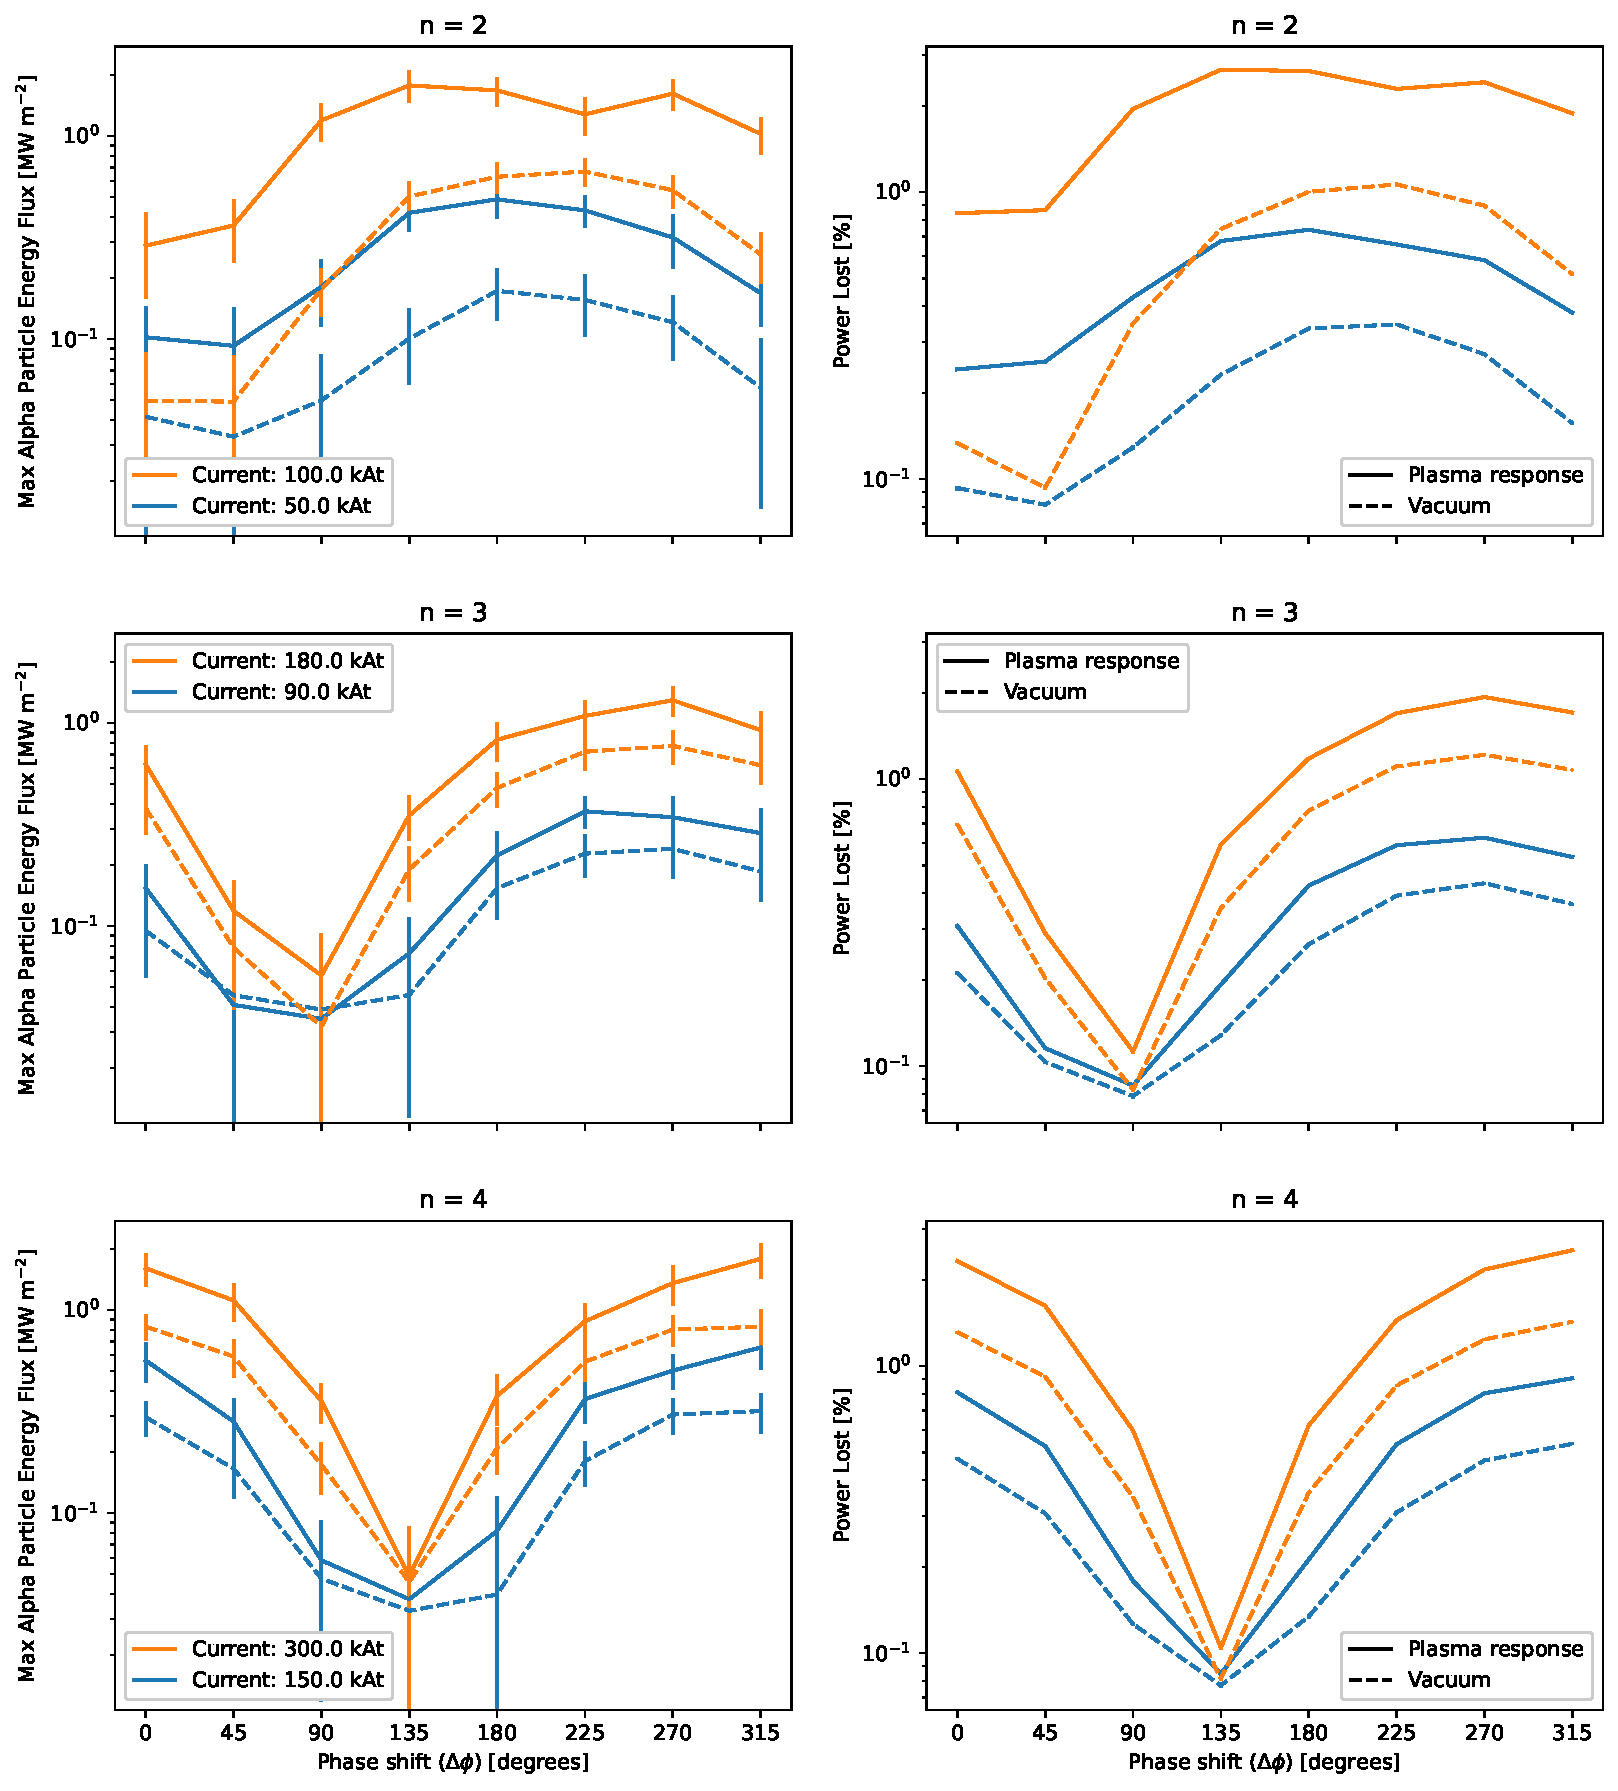
\includegraphics[width=0.99\linewidth]{Figures/max_and_total_flux_vs_phase.pdf}
    % \caption{Caption}
    % \caption{\parbox{0.9\linewidth}{This figure shows the results from 96 simulations. The left-columns s on the wall in $\si{MW.m^{-2}}$}}
    \caption{Maximum $\alpha$-particle energy flux on the first wall (left plots) and percentage loss of $\alpha$-particle power (right plots) for different ELM suppression coil parameters.}
    \label{fig:max_and_total_flux_vs_phase}
\end{figure}

The optimal $\Delta\phi$ for ELM suppression has been estimated using MARS-F by applying the criterion that the normalised field perturbation in the plasma should exceed $10^{-4}$: this has been found to be required for effective ELM control in current experiments. In the case of $n = 3$, with the plasma response included, it has been found that ELM suppression is favoured when $\Delta\phi \sim 180^{\circ}$, a value that is somewhat greater than the optimum for minimising $\alpha$-particle losses ($\sim 90^{\circ}$) in this case (see middle row of Fig. \ref{fig:max_and_total_flux_vs_phase}). The choice of $\Delta\phi$ may thus require a compromise between the requirements of ELM suppression and acceptably low $\alpha$-particle losses.  

In Fig. \ref{fig:energy_flux_distribution}, we look in more detail at one of the more conservative but likely scenarios where $n=3$, $I_0= 180\si{.kAt}$, $\Delta \phi = 90^\circ$ and where the plasma response is included. More precisely, Fig. \ref{fig:energy_flux_distribution} shows how the $\alpha$-particle energy flux is distributed along the wall. It shows the maximum energy flux of the $\alpha$-particles over all values of $\phi$ as a function of the poloidal distance along the wall ($s_\theta$), i.e.
\begin{equation}
    S_{max}(s_\theta) = \max_{0\le \phi \le 2\pi}\qty{S(\phi, s_\theta)},
\end{equation}
where $S=S(\phi, s_\theta)$ denotes the $\alpha$-particle energy flux on the first wall.
In the right-hand plot of Fig. \ref{fig:energy_flux_distribution}, the boundaries between the outboard and inboard walls and the upper and lower divertors are marked by vertical lines in blue, orange, green, and red. These are labeled with the symbols +, $\times$, $\bullet$, and $\blacksquare$ respectively. The corresponding symbols and colors are also shown in the left plots for reference. This shows that the largest peak is on the dome in the upper divertor with another significant peak at the end of the outer leg in the lower divertor.

\begin{figure}[!htb]
    \centering
    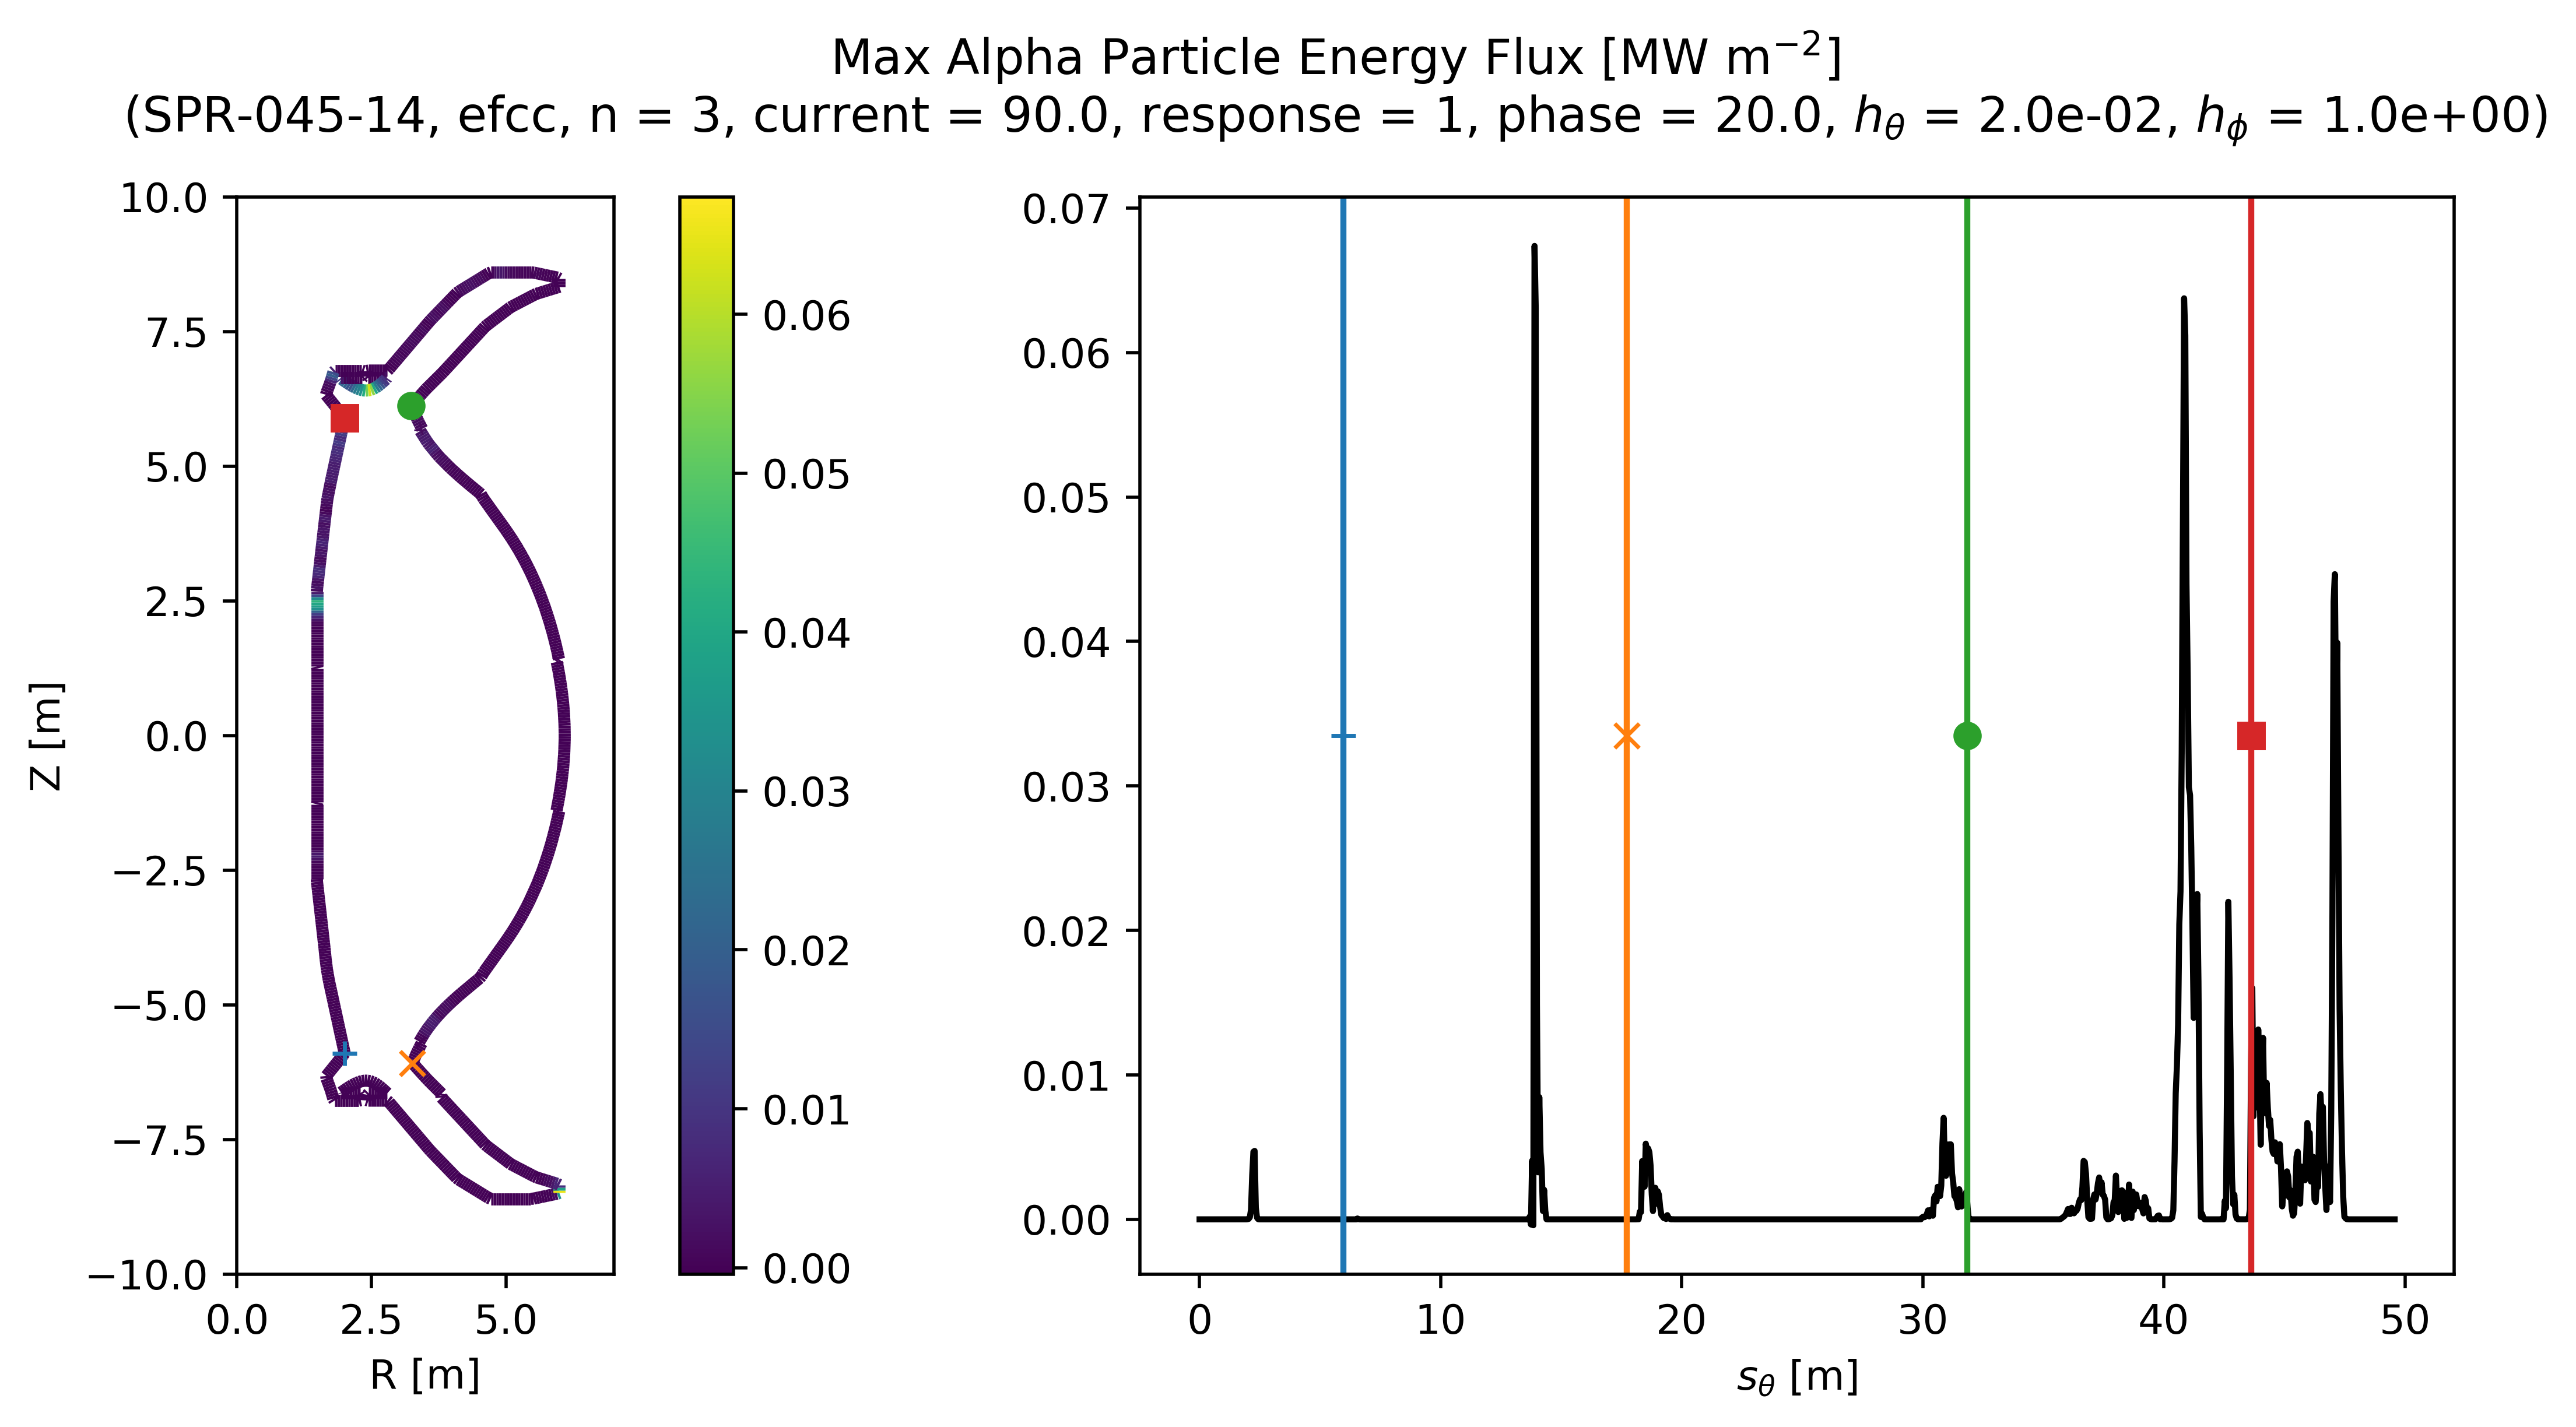
\includegraphics[width=0.7\linewidth]{Figures/simple_line_plot_no_confidence_band.png}
    \caption{Distribution of peak $\alpha$-particle energy flux maximised over toroidal angle in poloidal cross-section (left) and versus poloidal distance $s_\theta$ along the wall (right plot).}
    \label{fig:energy_flux_distribution}
\end{figure}

\section{TAE stability calculations}
\label{sec:halo_work}

TAEs are driven unstable due to wave-particle resonances, principally the Landau resonance that occurs when the particle speed parallel to the magnetic field matches the Alfv\'en speed, $c_A$. The only trans-Alfv\'enic fast ions of any significance in STEP DT plasmas will be the $\alpha$-particles, born with an approximately isotropic velocity distribution clustered around a speed ($\sim 1.3\times10^7\si{ms^{-1}}$). This is nearly an order of magnitude higher than typical values of $c_A$ envisaged in STEP flat-top operation, and therefore the resonance condition will be satisfied by $\alpha$-particles as they slow down. However, although the intrinsic fast ion drive of TAEs is expected to be high in STEP, strong bulk plasma damping of these modes is also expected. The reason for this is that STEP will need to be a high plasma $\beta$ device to generate net electrical power, and local values of $\beta$ in the plasma core may be a substantial fraction of unity, meaning that the bulk ion thermal speed $v_i$ will be comparable to $c_A$. Moreover, in addition to the primary Landau resonance $v_{\parallel}=c_A$, in a toroidal plasma there are also sideband resonances $v_{\parallel} = c_A/\vert 2\ell-1 \vert$ where $\ell$ is a positive integer. As a result of these two effects, many bulk ions as well as fast ions can resonate with TAEs in STEP plasmas, and the interaction of bulk ions with these modes is generally expected to result in strong Landau damping.

The stability of TAEs in STEP has been studied using the HAGIS \cite{pinches1998} and HALO \cite{fitzgerald2020} codes. One particular STEP scenario is relatively compact with major radius $R_0 = 3.0\,$m, toroidal field $B_0 = 1.8\,$T and central fuel ion temperature $T_i(0)=17\,$keV. Intrinsic growth rates (i.e. $\alpha$-particle drive) of TAEs with a range of values of $n$ in the absence of all damping processes are plotted in Fig. \ref{fig:TAEs}. It can be seen that most TAEs have normalised growth rates $\gamma/\omega$ of a few percent but one $n=2$ mode has much stronger drive, with $\gamma/\omega \simeq 0.18$. In this case, the mode electric field extends further into the plasma core than that of other modes and can thus interact with a high concentration of $\alpha$-particles deep inside the plasma. 

\begin{figure}[!htb]
    \centering
    \vskip -3.0cm
    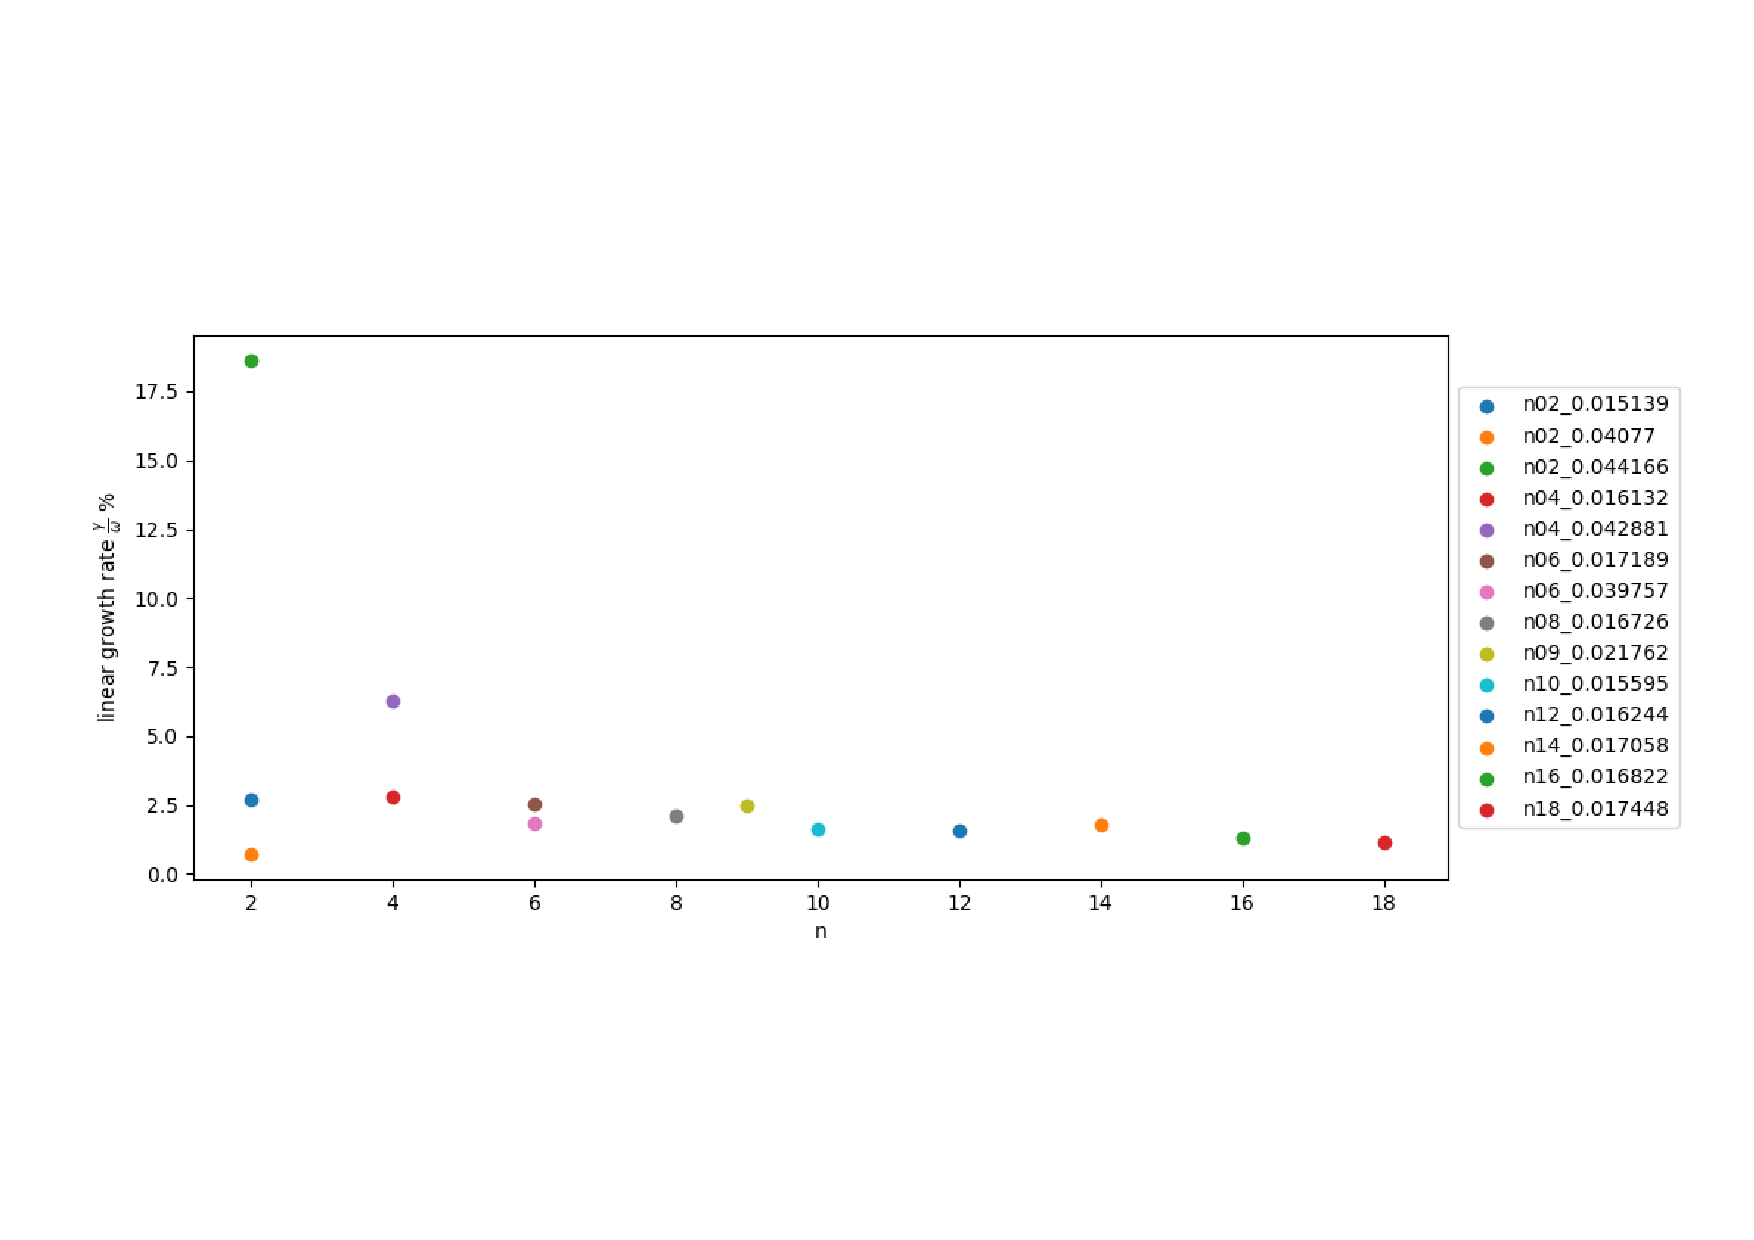
\includegraphics[width=1.0\linewidth]{Figures/TAE_figure.pdf}
    \vskip -3.0cm
    \caption{Growth rates of TAEs with damping neglected in equilibrium with $B_0 = 1.8\,$T, $T_i(0) = 17\,$keV computed using HAGIS. The legend indicates the mode $n$ and squared frequency normalised to $c_A/R_0$ where $c_A$ is the Alfv\'en speed at the magnetic axis, $R=R_0$.}
    \label{fig:TAEs}
\end{figure}

HALO calculations indicate that bulk ion Landau damping of this mode $\gamma_d$ is even stronger than the drive: we find that $\gamma_d/\omega \simeq -1.4$. It should be noted that this damping rate is exponentially sensitive to the bulk ion plasma beta, and therefore it is important to carry out a sensitivity scan of the plasma parameters, in particular $B_0$ and $T_i(0)$. We find however that TAEs remain damped in other flat-top plasma scenarios.        

\section{Discussion, conclusions and future study}
\label{sec:discussion_and_conclusions}

As expected, $\alpha$-particles in STEP are well-confined in the axisymmetric limit, and TF ripple losses are acceptably low if there are 16 TF coils with outer limbs at major radii of at least $\si{8.m}$. Losses arising from the use of ELM suppression coils pose a more substantial challenge. Our work demonstrates that a sub-optimal choice of phase difference $\Delta\phi$ between the upper and lower sets of ELM coils can result in significant deterioration of the $\alpha$-particle confinement, and the optimum $\Delta\phi$ for ELM suppression does not coincide with that for $\alpha$-particle confinement. Further experimental research in spherical tokamaks is needed in order to establish the requirements of active ELM suppression in STEP. Nevertheless, the work presented here provides useful insights to inform the design process, giving us more confidence that a solution to the ELM problem that is compatible with acceptable $\alpha$-particle losses can be found.

To maximise the fusion power, it is intended that STEP will operate above the no-wall beta limit for resistive wall modes (RWMs) with $n=1$. Active and passive control of RWMs will therefore be required \cite{xia2023}. When noise is taken into account, residual field perturbations with dominant $n=1$ are present during RWM control, and these perturbations have the potential to degrade $\alpha$-particle confinement. We therefore plan to model the effects of residual field perturbations due to dedicated RWM coil currents on $\alpha$-particle confinement. The most recent STEP design includes 8 RWM active control coils along the midplane. Toroidal sidebands, discussed in Section \ref{sec:elm_suppression_field}, will make up a significant part of the RWM field and will therefore need to be included in the LOCUST modelling.

It is intended that future work in the area of Alfv\'en eigenmode stability in STEP will focus on possible destabilisation of these modes by fast electrons during the ramp-up phase (when electron cyclotron current drive will be used \cite{freethy2023}) and by runaway electrons during disruptions, while in the flat-top phase the dependence of Alfv\'en eigenmode stability on the $q$-profile will be investigated. 

\section*{Acknowledgements}

This work has been funded by STEP, a UKAEA program to design and build a prototype fusion energy plant and a path to commercial fusion.

% Format text for bibliography
% If more than three authors put et al.
\fontsize{9}{12}\selectfont
\setlength{\parskip}{0pt}
\begin{thebibliography}{9}

\bibitem{nuttall2020} % book chapter
% example: CHAPTER-AUTHOR, A., “Title of chapter in sentence case”, Book Title in Title Case, Publisher, Place of Publication (Year).
    WILSON, H., CHAPMAN, I., DENTON, T., et al., 
    ``STEP---on the pathway to fusion commercialization", 
    Commercialising Fusion Energy, 
    IOP Publishing, 
    (2020).

\bibitem{meyer2023} % poster at conference
% example: PRESENTER, A., “Title of presentation in sentence case”, Paper No., paper presented at Organization seminar on subject, Location, year.
    MEYER, H.,
    ``The plasma scenarios for the Spherical Tokamak for Energy Production (STEP) and their technical implications",
    29\textsuperscript{th} IAEA Fusion Energy Conference,
    poster presentation, 
    London, UK, 
    2023

\bibitem{mitchell2023} % journal article
% example: AUTHOR, A., AUTHOR, B., AUTHOR, C., Journal article title in sentence case, Abb. J. Title 1 2 (Year) 120–123.
    MITCHELL, J., PARROTT, A., CASSON, F., et al.,
    Scenario trajectory optimization and control on STEP,
    Fusion Eng. Des.
    \textbf{192} 
    (2023) 
    113777.

\bibitem{garcia-munoz2011} % journal article
% example: AUTHOR, A., AUTHOR, B., AUTHOR, C., Journal article title in sentence case, Abb. J. Title 1 2 (Year) 120–123.
    GARC\'IA-MU\~NOZ, M., CLASSEN, I.G.J., GEIGER, B., et al., 
    Fast ion transport induced by Alfv\'en eigenmodes in the ASDEX Upgrade tokamak, 
    Nucl. Fusion 
    \textbf{51} 
    (2015) 
    103013.

\bibitem{bachmann2018} % internal report
% example: AUTHOR, A., Internal Report Title in Title Case, internal report, Organization, Location, Year.
    BACHMANN, C., CIATTAGLIA, S., CISMONDI, F., et al., 
    Overview over DEMO design integration challenges and their impact on component design concepts, 
    Fusion Eng. Des. 
    \textbf{136} 
    (2018)
    87.

\bibitem{fil2023} % poster at conference
% example: PRESENTER, A., “Title of presentation in sentence case”, Paper No., paper presented at Organization seminar on subject, Location, year.
    FIL, A., HENDEN, L., NEWTON, S., et al.,
    ``Disruption runaway electron generation and mitigation in the Spherical Tokamak for Energy Production",
    poster presentation, 
    29\textsuperscript{th} IAEA Fusion Energy Conference,
    London, UK, 
    2023

\bibitem{zohm1996} % journal article
% example: AUTHOR, A., AUTHOR, B., AUTHOR, C., Journal article title in sentence case, Abb. J. Title 1 2 (Year) 120–123.
    ZOHM, H., 
    Edge localized modes (ELMs), 
    Plasma Phys. Control. Fusion 
    \textbf{38} 2 
    (1996) 
    105.

\bibitem{suttrop2018} % journal article
% example: AUTHOR, A., AUTHOR, B., AUTHOR, C., Journal article title in sentence case, Abb. J. Title 1 2 (Year) 120–123.
    SUTTROP, W., KIRK, A., BOBKOV, V., et al.,
    Experimental conditions to suppress edge localised modes by magnetic perturbations in the ASDEX Upgrade tokamak,
    Nucl. Fusion,
    \textbf{58} 9 
    (2018) 
    096031.
    
\bibitem{van2015} % journal article
% example: AUTHOR, A., AUTHOR, B., AUTHOR, C., Journal article title in sentence case, Abb. J. Title 1 2 (Year) 120–123.
    VAN ZEELAND, M., FERRARO, N., GRIERSON, B., et al.,
    Fast ion transport during applied 3D magnetic perturbations on DIII-D,
    Nucl. Fusion,
    \textbf{55} 7,
    (2015)
    073028.

\bibitem{sanchis2018} % journal article
% example: AUTHOR, A., AUTHOR, B., AUTHOR, C., Journal article title in sentence case, Abb. J. Title 1 2 (Year) 120–123.
    SANCHIS, L., GARCIA-MUNOZ, M., SNICKER, A., et al.,
    Characterisation of the fast-ion edge resonant transport layer induced by 3D perturbative fields in the ASDEX Upgrade tokamak through full orbit simulations,
    Plasma Phys. Control. Fusion,
    \textbf{61} 1,
    (2018)
    014038.
    
\bibitem{ward2022} % journal article
% example: AUTHOR, A., AUTHOR, B., AUTHOR, C., Journal article title in sentence case, Abb. J. Title 1 2 (Year) 120–123.
    WARD, S., AKERS, R., LI, L., et al.,
    LOCUST-GPU predictions of fast-ion transport and power loads due to ELM-control coils in ITER,
    Nucl. Fusion,
    \textbf{62} 12
    (2022)
    126014.

\bibitem{akers2018} % poster at conference
    % example: PRESENTER, A., “Title of presentation in sentence case”, Paper No., paper presented at Organization seminar on subject, Location, year.
    AKERS, R., COLLING, B., HESS, J., et al.,
    ``High fidelity simulations of fast ion power flux driven by 3D field perturbations on ITER",
    poster presentation, 
    26\textsuperscript{th} IAEA Fusion Energy Conference,
    Kyoto, Japan, 
    2016.

\bibitem{ward2021} % journal article
% example: AUTHOR, A., AUTHOR, B., AUTHOR, C., Journal article title in sentence case, Abb. J. Title 1 2 (Year) 120–123.
    WARD, S., AKERS, R., JACOBSEN, A., et al.,
    Verification and validation of the high-performance Lorentz-orbit code for use in stellarators and tokamaks (LOCUST),
    Nucl. Fusion,
    \textbf{61} 8
    (2021)
    086029.

\bibitem{bosch1992} % journal article
% example: AUTHOR, A., AUTHOR, B., AUTHOR, C., Journal article title in sentence case, Abb. J. Title 1 2 (Year) 120–123.
    BOSCH, H., HALE, G.,
    Improved formulas for fusion cross-sections and thermal reactivities,
    Nucl. Fusion,
    \textbf{32} 4
    (1992)
    611-631.

\bibitem{brysk1973} % journal article
% example: AUTHOR, A., AUTHOR, B., AUTHOR, C., Journal article title in sentence case, Abb. J. Title 1 2 (Year) 120–123.
    BRYSK, H.,
    Fusion neutron energies and spectra,
    Plasma Phys.,
    \textbf{15} 7
    (1973)
    611-617.

\bibitem{chen2017} % journal article
% example: AUTHOR, A., AUTHOR, B., AUTHOR, C., Journal article title in sentence case, Abb. J. Title 1 2 (Year) 120–123.
    CHEN, Yen-Chi,
    A tutorial on kernel density estimation and recent advances,
    Biostat. Epidemiol,
    \textbf{1} 1
    (2017)
    161-187.

\bibitem{mcclements2005} % journal article
% example: AUTHOR, A., AUTHOR, B., AUTHOR, C., Journal article title in sentence case, Abb. J. Title 1 2 (Year) 120–123.
    MCCLEMENTS, K.,
    Full orbit computations of ripple-induced fusion $\alpha$-particle losses from burning tokamak plasmas,
    Phys. of Plasmas,
    \textbf{12} 7
    (2005)
    072510.

\bibitem{liu2015} % journal article
% example: AUTHOR, A., AUTHOR, B., AUTHOR, C., Journal article title in sentence case, Abb. J. Title 1 2 (Year) 120–123.
    LIU, Y., AKERS, R., CHAPMAN, I., et al.,
    Modelling toroidal rotation damping in ITER due to external 3D fields,
    Nucl. Fusion,
    \textbf{55} 6
    (2015)
    063027.

\bibitem{pinches1998} % journal article
% example: AUTHOR, A., AUTHOR, B., AUTHOR, C., Journal article title in sentence case, Abb. J. Title 1 2 (Year) 120–123.
    PINCHES, S.D., APPEL, L.C., CANDY, J., et al.,
    The HAGIS self-consistent nonlinear wave-particle interaction model,
    Computer Phys. Commun.
    \textbf{111}
    (1998)
    133.

\bibitem{fitzgerald2020} % journal article
% example: AUTHOR, A., AUTHOR, B., AUTHOR, C., Journal article title in sentence case, Abb. J. Title 1 2 (Year) 120–123.
    FITZGERALD, M., BUCHANAN, J, AKERS, R.J., et al.,
    HALO: a full-orbit model of nonlinear interaction of fast particles with eigenmodes,
    Computer Phys. Commun.
    \textbf{252}
    (2020)
    106773.

\bibitem{xia2023} % journal article
% example: AUTHOR, A., AUTHOR, B., AUTHOR, C., Journal article title in sentence case, Abb. J. Title 1 2 (Year) 120–123.
    XIA, G., LIU, Y., HENDER, T., et al.,
    Control of resistive wall modes in the spherical tokamak,
    Nucl. Fusion,
    \textbf{63} 2
    (2023)
    026021.

\bibitem{freethy2023} % poster at conference
% example: PRESENTER, A., “Title of presentation in sentence case”, Paper No., paper presented at Organization seminar on subject, Location, year.
    FREETHY, S.,
    ``The STEP microwave heating and current drive system",
    29\textsuperscript{th} IAEA Fusion Energy Conference,
    poster presentation, 
    London, UK, 
    2023

\end{thebibliography}


\end{document}
